\section{The Heart}

The heart's role is to pump blood around the body, driving the circulation of
the blood and everything contained within it.  It is one of the most important
organs in the body and any malfunction in its behaviour could be fatal in very
short order.  It begins beating in the early stages of pregnancy and continues
until death, hopefully many decades later.  It beats at an average rate of
around 70 beats per minute (bpm) for the adult male and 75 bpm for the adult
female.

The heart is not, as popular belief would have it, the seat of human emotion.
The functioning of the heart is modulated by such emotion however, slowing when
we are calm and increasing in rate quite dramatically when we are excited or
afraid.  Despite being influenced by the brain and our emotional states, the
heart drives itself, rather than having the pace-making initiated outside the
organ.

\subsection{Location of the Heart}

The human heart sits in the centre of the chest, the bulk of it extending into the
left-hand side of the chest cavity, inside a fibrous sac called the pericardium.
The actual location, orientation and size can vary quite significantly from
individual to individual~\cite{Oberman1967}.


\subsection{Gross Structure of the Heart}

The heart is mostly muscle.
This muscle is anchored to a collagenous `skeleton', known as the annulus
fibrosus located at the atrio-ventricular junction.
The muscle is different from the `smooth' skeletal muscle, in both structure
and behaviour~\cite{Katz2006}.

The human heart has four chambers; two atria and two ventricles.  The atria receive
the blood from the circulatory system and force it into the two ventricles,
which then contract and force this blood out and around the lungs and body.
These chambers are known as the left and right atria and the left and right
ventricles.  The left hand side of the heart in humans is much more developed
than the right.
This is due to their differing roles in circulating the blood.

The right and left atria are smaller than their respective ventricles and have
much thinner walls, because they need to develop much less pressure.  The right
atrium receives the blood from the circulatory system which is de-oxygenated,
and passes it on to the right ventricle.  The left atrium receives the highly
oxygenated blood from the lungs, and passes it onto the left ventricle.  The two
atria are separated by a thin muscle wall known as the intra-atrial septum.
This prevents the mixing of blood between the two atrial chambers.

The differences between the right and left ventricles are much more pronounced
than those between the right and left atria.  The right ventricle must merely
pump blood around the lungs and developing too high a pressure there could
actually damage the delicate structures.  By contrast the left ventricle must
develop enough pressure to drive blood around the whole body and as such it is
much more muscular.  The two ventricles are divided by the ventricular
septum.

As noted earlier, separating the atria and ventricles is the annulus fibrosus
or central fibrous body.
This is a dense layer of fibrous tissue.
In addition to providing an anchor for the muscle of the heart, it electrically
isolates the atria from the ventricles.
In the normal heart, the only electrical connection between the atria and the
ventricles is at the atrio-ventricular node.
This connects the right atrium to the specialist conduction system of the
ventricles.

\subsection{The Atria}

Examination of the human atria (or auricles, in older literature) is as old as studies
of the heart.
However, in recent years there has been a renewed interest in the
atria and their structures.
This has followed an increasing appreciation that the atria are not merely
reservoirs of venous blood, but have an active role to play in the function of
the heart~\cite{Ho2002a,Ho2002b,Ho2009,Platonov2007,Platonov2008a}.

Descriptions of the location of features use the `altitudinal' description, where
this is possible.
Altitudinal descriptions use the coordinates of the body, such that `right' is
the body's right hand side, not the right of the observer.
In this description, the atria are located to the right of the ventricles.
They can be slightly superior, too.
The right atrium is anterior and to the right, the left atrium more posterior and to
the left of the body.

The atria have a number of common features.
Both have a valve on the base, which is part of the central fibrous body.
In the right atrium, this is the tricuspid valve, in the left, the mitral valve.
These valves feed into the respective ventricles.

Both atria also have appendages, although the appendages differ in form.
The right atrial appendage is large, with a triangular shape and a wide base.
It is located anteriorly and superiorly on the right atrium.
By contrast, the left atrial appendage is smaller and more tubular in nature.
It is located posteriorly and superiorly compared to the left atrium.

\subsubsection{The Right Atrium}

The right atrium gathers in blood from the body, after it has cycled around the
organs.
The right atrium has a simpler topology than the left atrium.
At the top is an opening for the superior vena cava, and at the base there are
openings for the inferior vena cava and the tricuspid valve.

The right atrium is the location of many of the important sites of the
conduction system of the heart.
The sinus node, or sino-atrial node (SAN), is located on the right atrial wall,
close to the superior vena cava.
The SAN is the primary pacemaker for the heart in normal function.
It achieves this through specialised cells, known as nodal cells.
These cells are what are termed `auto-active' and are capable of spontaneously
exciting.

Running down the lateral wall is a muscle ridge, known as the crista terminalis,
or terminal crest.
The crista terminalis delineates the smooth and rough parts of the right atrial
wall.
This muscle ridge consists mostly of myocytes---cardiac muscle cells---arranged
longitudinally along the main axis of the ridge, and so forms a path of
preferential conduction.
In addition, these cells have a specialised electrophysiology~\cite{Feng1998}.

At the inferior end of the crista terminalis there is the atrio-ventricular
node (AVN).
This is another area of specialised nodal cells.
These cells are also auto-active, although with a slower natural frequency than
the SAN.
They therefore only take over in the case of SAN failure.
The AVN is the only point of electrical contact between the atrium and
ventricles in the normal heart.
As well as providing a link between the atria and ventricles this region acts
to limit the rate of stimulus which is passed on to the ventricles, protecting
them from excessive atrial pacing rates.

Branching from the crista terminalis and spreading around the muscle wall of the
right atrium are the pectinate muscles.
Like the crista terminalis, these bundles consist mostly of cells lying end to
end, forming pathways of preferential conduction.
The conformation of the pectinate muscles varies between individuals; some have
complex branching and interwoven patterns, whilst others have simpler and
relatively parallel bundles.

\subsubsection{The Atrial Septum}

The atrial septum divides the two atria.
Much of the septum is actually an in-folding of the right atrium.
The true septum is limited to the fossa ovalis and the muscle ring immediately
surrounding it.
The fossa ovalis is a valve which is important in fetal circulation, but is
closed in the normal adult.
The fossa ovalis is mostly fibrous in nature.
The muscle fibres run in a predominately circular direction around the fossa.

\subsubsection{The Left Atrium}

The left atrium gathers blood from the lungs.
The pulmonary veins tend to give the left atrium a more complex topology than
the right.
This complex topology can make the pulmonary veins a source of arrhythmic
activity.

Unlike the right atrium, the left atrium is not dominated by the appendage.
In the left atrium, the appendage is small and largely separate from the main
body of the atrium.
The endocardial surface of the appendage is covered in many fine muscle ridges.
Between these ridges, the walls of the atrium can be paper thin.

Conventionally the left atrium is depicted as having four openings for the
pulmonary veins.
Recent studies, reviewed in~\cite{Ho2009}, suggest considerably more variation
with approximately one third of hearts having merged veins on one or both sides.
In some cases, the single vein can actually link all the way to the lungs.
The pulmonary veins are surrounded by a sheath of tissue.
There is evidence that cells in the sheaths can have different electrophysiology
to normal atrial cells~\cite{Jones2008}.

The left atrial wall is relatively smooth.
However, it is not uniform in thickness or muscle architecture.
It instead has a complex and overlapping muscle structure.
This can look like layers, but there are no insulating fibrous sheets between
bundles.

\subsubsection{Inter-atrial Connections}

The atria are linked by muscle bundles.
These muscle bundles have cells mainly oriented end to end, which gives
preferential conduction along their axis.
The most well known of these is the Bachmann's bundle, which is located
anteriorly and superiorly between the two atria.

Common thought has it that the Bachmann's bundle is the principle electrical
connection between the atria in sinus rhythm.
However, recent studies (summarised in~\cite{Platonov2007,Platonov2008a}) have
found that in a significant fraction of the population, a secondary pathway
which is inferior and/or posterior is used instead.
In some subjects, a Bachmann's bundle cannot even be located.
There are a lack of studies performed on healthy subjects, however, so it is
unclear what occurs in the normal case.

\subsection{Cardiac Myocytes}

Myocytes, or muscle cells, comprise the vast bulk of cardiac tissue.
They both conduct electrical signals and contract to provide the force needed to
pump the blood around the body.
This is accomplished by a complex interplay of ionic
currents~\cite{Katz2006}.

\subsubsection{Myocyte Structure}

A typical human myocyte is from 50 to 150$\,\mu$m long, and has a radius
between 10 and 20$\,\mu$m.
They have a roughly cylindrical shape.
The cell is wrapped in an impermeable membrane, called the sarcolemma or plasma
membrane.
The membrane in many myocytes is invaginated at various points by series of
fine transverse tubules (T tubules) that carry action potentials deep into the
myocytes.

The cellular membrane contains a large number of specialised structures
responsible for allowing a regulated flow of ions into and out of the cell.
These structures include passive channels, active pumps and gated channels.
They are used to modulate the ionic composition of the intracellular
space and play a vital role in modulating the electrical activity of the cell.
Because it is impermeable a potential difference can build across the membrane
between the inside and outside of a cell.
This is the membrane potential.

Within the cells, much of the space is filled with what are called
myofibril-like units, long branching fibres about 1$\mu$m in diameter.
These fibres are divided up into sarcomeres, approximately 2$\mu$m long in the
resting myocyte, which is considered the basic contractile unit.
Mitochondria, which provide the ATP needed to provide energy for the
contractions, also occupy a significant fraction of the intracellular space.
Mitochondria are not actually a part of the body in the strictest sense and
have their own DNA -- they are symbiotic organisms that entered our own cells
at some unknown time in the past.
One other structure within the cells that is important to the electrical and
mechanical behaviour of the cells is a second tubule network, known as the
sarcoplasmic reticulum (SR) and the sarcotubular network.
The SR stores calcium in subsarcolemmal cisternae, which is released during the
membrane depolarisation.
The cisternae form structures known as dyads (or diads) with the T tubules.

\subsubsection{Ion Channels and Pumps}

The structures in the cellular membrane which permit ions to cross can
be roughly divided into channels and pumps.
Most channels and pumps are specific to one specific ion type.
Channels passively allow ions to flow with the concentration gradient, whilst
pumps actively move ions, regardless of the gradient~\cite{Hille2001}.

Channels and pumps are classified by the ion(s) they transport and how they are
controlled.
They are also classified on the direction of charge flow.
An inward current is one that would have the effect of a positive ion entering
the cell and could therefore also be caused by negatively charged ions exiting
the cell.
Inward currents act to increase the potential in the cell.
Conversely, outward currents are those that would have the effect of a positive
ion leaving the cell.
They are repolarizing currents as they act to decrease the membrane potential.

Inter-cardiac current flows through the gap junctions, which allow for large
current flows.
These are formed at the centre of membrane structures known as intercalated
disks.
The intercalated disks are concentrated at the ends of cells, although there are
some transverse connections.

Channels rely on an ionic gradient to drive flow through them.
Some channels have a constant conductance.
These are typically called background currents.
Channels with a conductance which depend on the instantaneous membrane potential
are known as voltage-gated channels.
Other channels can have their conductance modulated by the presence of a
hormone or chemical, such as the ATP sensitive potassium channel.
\begin{figure}
\begin{center}
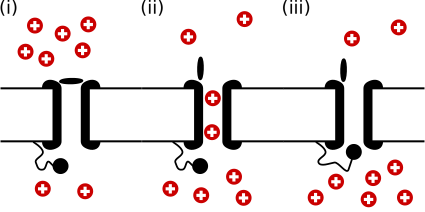
\includegraphics{figures/intro/activation_gate}
\end{center}
\caption[Time-Dependent Ion Channel]{
\label{fig:intro:heart:gated_ion}
A time dependant ion channel, represented by the black structure which bisects
the membrane (horizontal lines) for positive ions, shown as red circles.
The channel has an activation gate, the black lozenge on the top of the
membrane and an inactivation gate, the ball and chain on the underside of the
membrane.
In panel (i) the gate is not activated and shows a large concentration of ions
on the upper side.
In panel (ii), the gate activates and ions flow down the channel to the region
of lower concentration.
In panel (iii), the inactivation gate has moved to close the channel and no more
ions flow.
}
\end{figure}
Many gated channels are what are known as time-dependent channels.
These channels have structures over one or both ends which modulate the total
conductance to open (activate) or close (inactivate) the channel.
This is illustrated in figure~\ref{fig:intro:heart:gated_ion}.
The time course of this activation or inactivation is normally modulated by the
voltage, but can also be modulated by ion concentration or other mechanisms.
\begin{figure}
\begin{center}
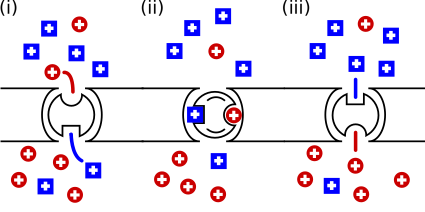
\includegraphics{figures/intro/ion_pump}
\end{center}
\caption[Ion Pump]{
\label{fig:intro:heart:ion_pump}
An ion pump (or more accurately, an ion exchanger), represented by the black
structure which bisects the membrane (horizontal lines) for two species of
positive ion, represented by red circles and blue squares.
The pump works against the concentration gradient.
In panel (i), the two ions bind to their respective sites on the pump.
In panel (ii), the pump changes its structure, drawing each ion through the
membrane.
In panel (iii), the pump releases the binding of the ions, letting them rejoin
the free ion populations.
}
\end{figure}
Pumps use energy to actively move ions against the gradient.
Complex molecules latch onto the ions on one side of the membrane and move them
through to the other side.
Many pumps are actually exchangers, which take in ions of one sort on one side
whilst transporting another type of ion the other way.

\subsubsection{Myocyte Electrical Action Potentials}

The evolution of the electrical state of the cell, from polarised to depolarised
and back again is termed the action potential (AP).
The shape and duration of
the action potential is mostly determined by the channels, carriers and pumps
across the cellular membrane, though the internal and external concentrations of
several ions and molecules can also have a significant effect.
There are three
principle ion species involved in the development of the action potential;
sodium ($\text{Na}^{\text{+}}$), potassium ($\text{K}^{\text{+}}$) and calcium
($\text{Ca}^{\text{2+}}$).
The third, calcium, is also important for contractile function.
Chlorine ($\text{Cl}^{\text{-}}$) is also of importance in some cells.

\begin{figure}
\begin{center}
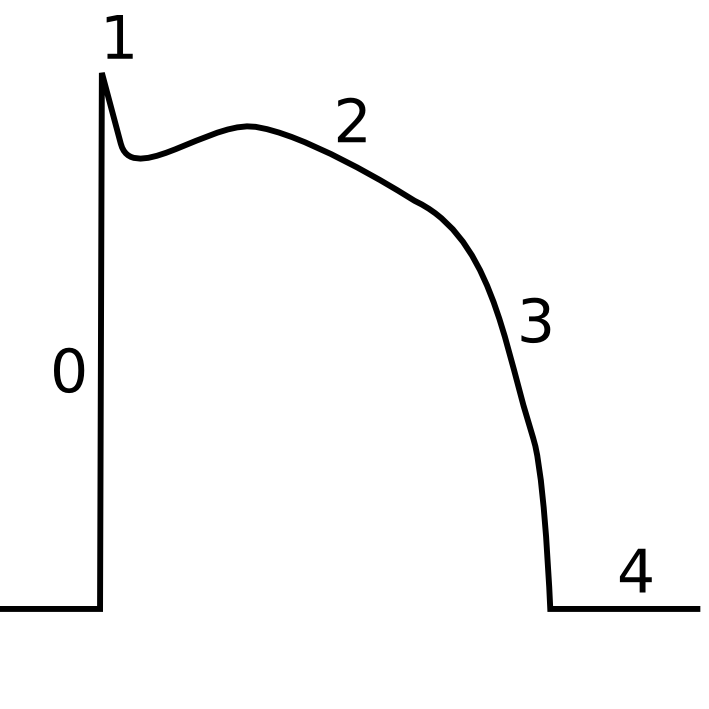
\includegraphics{figures/intro/ap_profile}
\end{center}
\caption[Schematic AP Profile]{
\label{fig:intro:heart:ap}
A schematic AP profile.
Labelled are the five phases of the action potential.
Phase 0, the upstroke.
Phase 1, the end of the upstroke.
Phase 2, the plateau.
Phase 3, the repolarization.
Phase 4, the resting period.
}
\end{figure}

The action potential has 5 phases (figure~\ref{fig:intro:heart:ap}).
It begins with depolarization, phase 0.
During depolarisation, the current is carried principally by the fast inward
sodium current.
Phase 0 is also known as the upstroke of the action potential, and its slope is
important to the propagation of the action potential through cardiac tissue and
also the excitability of the myocyte as in individual cell.
Phase 0 is over almost instantaneously in healthy myocytes.

Phase 1 signifies the end of the upstroke, and is caused by the inactivation of
the sodium channels.
The small notch present in some cellular action potentials is caused by a
transient net outward current, carried principally by potassium.

Phase 2 is the plateau phase.  This relatively long phase ($>$100ms in some
myocytes) is due to the balance of slowly activating inward calcium currents and
the outward potassium currents.
The inward calcium current is principally carried by the L-type calcium channels
and the outward potassium current by a plethora of channels, classified by the
speed of activation or the substance which modulates them.

Phase 3 is the repolarization period.
The calcium channels have inactivated.
The potassium currents are still open, and the net efflux of positive charge
repolarizes the cell.

The final phase 4 is the period during which the cell is at the resting
potential.
In addition, for a short period of phase 4, the cell is in fact
impossible to excite above this resting potential due to the inactivations of
numerous channels.
This is called the refractory period.

Both the shape and the length of the action potential have physiological
importance.
Many pathological conditions have a significant impact upon both.
The action potential duration (APD) is often given as an \apd\ or
\apd[50], denoting the duration of the AP at 90\% or 50\% repolarization,
respectively.
